\documentclass[
11pt, % The default document font size, options: 10pt, 11pt, 12pt
%codirector, % Uncomment to add a codirector to the title page
]{charter} 




% El títulos de la memoria, se usa en la carátula y se puede usar el cualquier lugar del documento con el comando \ttitle
\titulo{Sistema de monitoreo para equipos de captura de CO$_2$} 

% Nombre del posgrado, se usa en la carátula y se puede usar el cualquier lugar del documento con el comando \degreename
%\posgrado{Carrera de Especialización en Sistemas Embebidos} 
\posgrado{Carrera de Especialización en Internet de las Cosas} 
%\posgrado{Carrera de Especialización en Intelegencia Artificial}
%\posgrado{Maestría en Sistemas Embebidos} 
%\posgrado{Maestría en Internet de las cosas}

% Tu nombre, se puede usar el cualquier lugar del documento con el comando \authorname
\autor{Ing. Alena Grebneva} 

% El nombre del director y co-director, se puede usar el cualquier lugar del documento con el comando \supname y \cosupname y \pertesupname y \pertecosupname
\director{Mg. Ing. Milton Eduardo Sosa}
\pertenenciaDirector{FIUBA} 
% FIXME:NO IMPLEMENTADO EL CODIRECTOR ni su pertenencia
\codirector{John Doe} % para que aparezca en la portada se debe descomentar la opción codirector en el documentclass
\pertenenciaCoDirector{FIUBA}

% Nombre del cliente, quien va a aprobar los resultados del proyecto, se puede usar con el comando \clientename y \empclientename
\cliente{Mg. Ing. Eddie Jose Sierra Higuerey}
\empresaCliente{Green Backbone}

% Nombre y pertenencia de los jurados, se pueden usar el cualquier lugar del documento con el comando \jurunoname, \jurdosname y \jurtresname y \perteunoname, \pertedosname y \pertetresname.
\juradoUno{Nombre y Apellido (1)}
\pertenenciaJurUno{pertenencia (1)} 
\juradoDos{Nombre y Apellido (2)}
\pertenenciaJurDos{pertenencia (2)}
\juradoTres{Nombre y Apellido (3)}
\pertenenciaJurTres{pertenencia (3)}
 
\fechaINICIO{25 de abril de 2023}		%Fecha de inicio de la cursada de GdP \fechaInicioName
\fechaFINALPlan{13 de junio de 2023} 	%Fecha de final de cursada de GdP
\fechaFINALTrabajo{Marzo de 2024}	%Fecha de defensa pública del trabajo final


\begin{document}

\maketitle
\thispagestyle{empty}
\pagebreak


\thispagestyle{empty}
{\setlength{\parskip}{0pt}
\tableofcontents{}
}
\pagebreak


\section*{Registros de cambios}
\label{sec:registro}


\begin{table}[ht]
\label{tab:registro}
\centering
\begin{tabularx}{\linewidth}{@{}|c|X|c|@{}}
\hline
\rowcolor[HTML]{C0C0C0} 
Revisión & \multicolumn{1}{c|}{\cellcolor[HTML]{C0C0C0}Detalles de los cambios realizados} & Fecha      \\ \hline
0      & Creación del documento y asignación del director      &\fechaInicioName \\ \hline
1      & Se completa hasta el punto 5 inclusive                 & 8 de mayo de 2023 \\ \hline
%2      & Se completa hasta el punto 7 inclusive
%		  Se puede agregar algo más \newline
%		  En distintas líneas \newline
%		  Así                                                    & dd/mm/aaaa \\ \hline
%3      & Se completa hasta el punto 11 inclusive                & dd/mm/aaaa \\ \hline
%4      & Se completa el plan	                                 & dd/mm/aaaa \\ \hline
\end{tabularx}
\end{table}

\pagebreak



\section*{Acta de constitución del proyecto}
\label{sec:acta}

\begin{flushright}
Buenos Aires, \fechaInicioName
\end{flushright}

\vspace{1cm}

Por medio de la presente se acuerda con la \authorname\hspace{1px} que su Trabajo Final de la \degreename\hspace{1px} se titulará ``\ttitle'' y consistirá en el desarrollo de un prototipo para un sistema capaz de monitorear a distancia los equipos de captura de CO$_2$ pertenecientes al proyecto \textit{Green Backbone}, y tendrá un presupuesto preliminar estimado de 600 h de trabajo y \textcolor{red}{\$XXX}, con fecha de inicio el \fechaInicioName\hspace{1px} y fecha de presentación pública en \fechaFinalName.

Se adjunta a esta acta la planificación inicial.

\vfill

% Esta parte se construye sola con la información que hayan cargado en el preámbulo del documento y no debe modificarla
\begin{table}[ht]
\centering
\begin{tabular}{ccc}
\begin{tabular}[c]{@{}c@{}}Dr. Ing. Ariel Lutenberg \\ Director posgrado FIUBA\end{tabular} & \hspace{2cm} & \begin{tabular}[c]{@{}c@{}}\clientename \\ Fundador de \textit{\empclientename} \end{tabular} \vspace{2.5cm} \\ 
\multicolumn{3}{c}{\begin{tabular}[c]{@{}c@{}} \supname \\ Director del Trabajo Final\end{tabular}} \vspace{2.5cm} \\
%\begin{tabular}[c]{@{}c@{}}\jurunoname \\ Jurado del Trabajo Final\end{tabular}     &  & \begin{tabular}[c]{@{}c@{}}\jurdosname\\ Jurado del Trabajo Final\end{tabular}  \vspace{2.5cm}  \\
%\multicolumn{3}{c}{\begin{tabular}[c]{@{}c@{}} \jurtresname\\ Jurado del Trabajo Final\end{tabular}} \vspace{.5cm}                                                                     
\end{tabular}
\end{table}




\section{1. Descripción técnica-conceptual del proyecto a realizar}
\label{sec:descripcion}
El presente proyecto forma parte de la iniciativa de sostenibilidad \textit{Green Backbone} (en adelante GB) cuyo objetivo es hacer frente a los efectos de la emisión de gases de efecto invernadero (GEI) y descarbonizar el aire del ambiente. 

La emisión de GEI que se produce en actividades humanas, tales como la quema de hidrocarburos y la industrialización, se asocia con el cambio climático y tiene efectos significativos en los sistemas naturales y humanos en todo el mundo, por ejemplo, el aumento del nivel del mar, el derretimiento de glaciares y la alteración de los patrones climáticos. Estos efectos a su vez pueden tener un impacto importante en la seguridad alimentaria, en la disponibilidad de agua y en la salud humana. 

Para hacer frente a esta problemática algunos actores globales (países, compañías e instituciones) acordaron implementar estrategias para reducir paulatinamente la emisión de los GEI hacia el año 2030 y llegar al año 2050 con emisión cero (también conocido como \textit{net zero}). 

Sin embargo, estos esfuerzos han demostrado no ser suficientes y por ello en los último años han surgido iniciativas para el desarrollo de soluciones tecnológicas que permitan remover grandes cantidades de dióxido de carbono (entre 100 y 1.000 Gt de CO$_2$) presente en la atmósfera y alcanzar el \textit{net zero} más rápidamente.

El proyecto GB es liderado el Mg. Ing. Eddie Jose Sierra Higuerey y surgió en Bogotá (Colombia), en el año 2021, como uno de los participantes de la competencia global \textit{XPRIZE Carbon Removal}, donde se ofrecía un premio económico a quienes desarrollen y demuestren la eficiencia de soluciones tecnológicas para secuestrar y retener el dióxido de carbono (CO$_2$) de la atmósfera y los océanos.

Durante la competencia los miembros del equipo de GB desarrollaron un proceso químico innovador para capturar CO$_2$ del aire y demostró su funcionamiento en un prototipo de pequeña escala. En este proceso el aire del ambiente se inyecta con un compresor en un reactor que contiene desechos orgánicos y luego se lo hace circular por un tren de fotobiorreactores. El CO$_2$ queda retenido en ambas etapas del proceso y se puede comercializar como materia prima.

Para capturar grandes volúmenes de CO$_2$ mediante la implementación a gran escala del proceso químico desarrollado, el equipo de GB de Bogotá comenzó a construir en el año 2022 un prototipo comercial al que se denominó “GB005 Unidad Ángel”, que se estima que podrá capturar 3,3 toneladas de CO$_2$ al año. Esta unidad permitirá validar las tecnologías, mejorar el diseño y atraer inversionistas al proyecto.

Para la unidad GB005 se solicitó a la autora del proyecto desarrollar un dispositivo que registre y muestre en un display LCD los niveles de concentración de CO$_2$ en la entrada y la salida de aire del equipo, para evaluar el rendimiento del proceso de captura. 
A este dispositivo se adicionaron sensores de temperatura y pH para monitorear los biorreactores, así como un módulo sensor de luz y relés para controlar el encendido y apagado de la unidad. En la figura \ref{fig:diagNodo} se muestra el diagrama en bloques del dispositivo, al que se denomina nodo de medición. 

\begin{figure}[htpb]
\centering 
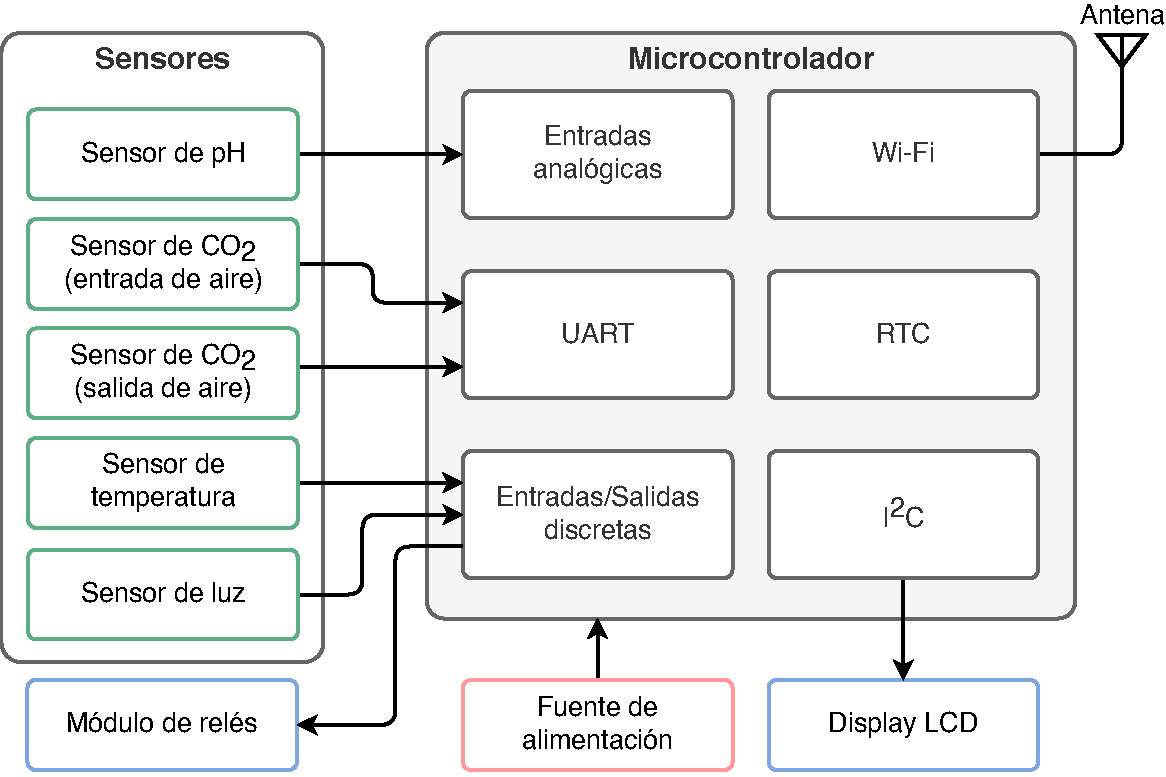
\includegraphics[width=.65\textwidth]{./Figuras/dgNodo.pdf}
\caption{Diagrama en bloques del nodo de medición.}
\label{fig:diagNodo}
\end{figure}

En una instancia de trabajo anterior al curso del posgrado se definió qué microcontrolador y sensores se van a utilizar y se propuso la conexión de todos los elementos. Asimismo, se desarrolló un firmware básico para poder monitorear los niveles de CO$_2$ y mostrar las mediciones en un display. En el presente proyecto se tomará esta base de diseño para mejorar el firmware propuesto.

A futuro, cuando se logre un diseño eficiente y se obtenga financiación, GB proyecta la construcción en serie de nuevas unidades en diferentes tamaños y capacidades de captura, para comercializar tanto en Colombia, como en el resto del mundo. Por ello, además del nodo de monitoreo para cada unidad, se necesita una plataforma capaz de recolectar y almacenar datos operativos de todas las unidades instaladas, sin importar donde se localicen físicamente.

Como la primera unidad de GB aún se encuentra en etapa de desarrollo, la propuesta del presente proyecto es un prototipo para evaluar su desempeño, agregar funciones de comunicación inalámbrica al nodo para que envíe las mediciones de los sensores hacia un broker MQTT (\textit{Message Queues Telemetry Transport}) y desarrollar la infraestructura del sistema de monitoreo.

En la figura \ref{fig:diagBloques} se muestra una arquitectura tentativa del sistema donde se tiene el nodo de medición, un broker MQTT donde se enviarán los datos de las mediciones y un entorno de desarrollo para la aplicación que leerá los datos del broker y con estos permitirá visualizar el funcionamiento general de la unidad, en tiempo real, a través del servidor de aplicación y almacenar la información operativa en una base de datos de tiempo real. 

\begin{figure}[htpb]
\centering 
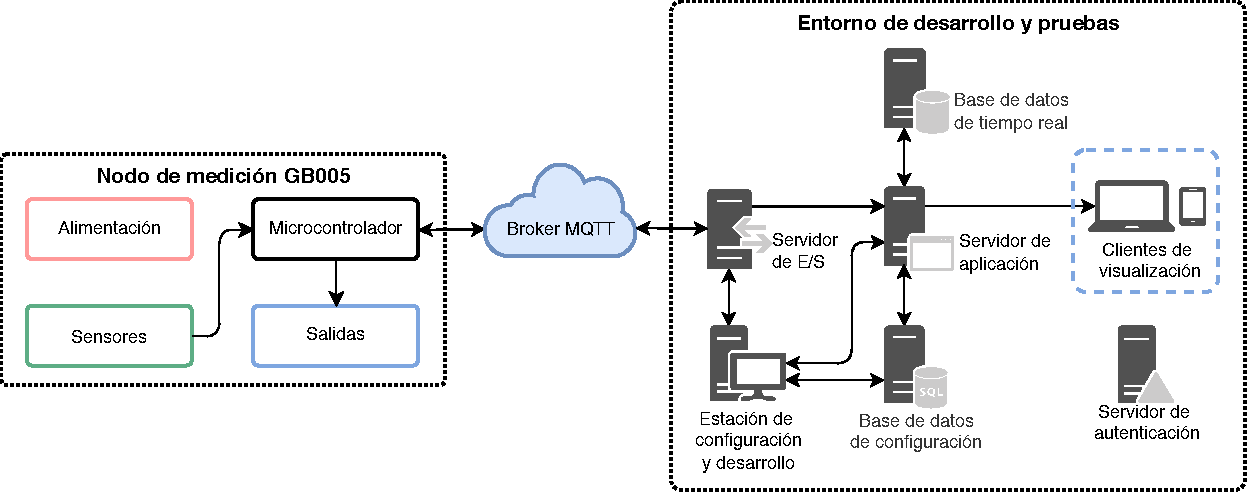
\includegraphics[width=1\textwidth]{./Figuras/diagBloques.pdf}
\caption{Arquitectura del sistema.}
\label{fig:diagBloques}
\end{figure}

\vspace{25px}

Actualmente existen diferentes soluciones de mercado para implementar aplicaciones IoT. En el presente proyecto, para desarrollar el sistema de monitoreo se empleará el software \textit{AVEVA System Platform} (ASP) ya que es una solución ampliamente utilizada en la industria con continuo desarrollo y soporte y está preparada para .

El ASP soporta el protocolo MQTT, tiene un entorno gráfico que permite la implementación de aplicaciones de visualización y una base de datos histórica para almacenar las mediciones de los sensores. Además por ser la autora del presente proyecto empleada de la empresa que comercializa la solución, tiene acceso a una licencia de desarrollo sin cargo, lo que permite reducir costos y tiempo de desarrollo del proyecto.

\section{2. Identificación y análisis de los interesados}
\label{sec:interesados}


\begin{table}[ht]
%\caption{Identificación de los interesados}
%\label{tab:interesados}
\begin{tabularx}{\linewidth}{@{}|l|X|X|l|@{}}
\hline
\rowcolor[HTML]{C0C0C0} 
Rol           & Nombre y Apellido & Organización 		& Puesto 	\\ \hline
%Auspiciante  & -                 & 			 		& -      	\\ \hline
Cliente       & \clientename      &\empclientename /AVEVA	&  Fundador de GB \\ \hline
%Impulsor     &                   &              		&        	\\ \hline
Responsable   & \authorname       & FIUBA   			& Alumna 	\\ \hline
Colaboradores & -                 & -            		& Empleados de GB/AVEVA \\ \hline
Orientador    & \supname	      	 & \pertesupname 		& Director del trabajo final \\ \hline
%Equipo       & miembro1 \newline 
%				miembro2        	 &              		&        	\\ \hline
%Opositores   &                   &              		&        	\\ \hline
Usuario final & -				 & -            		&  Equipo de GB y sus clientes\\ \hline
\end{tabularx}
\end{table}

\begin{itemize}
	\item Cliente: Eddie Sierra, creó GB como emprendimiento personal y es el principal interesado en el desarrollo de la aplicación de monitoreo para mostrar el valor del proyecto. Trabaja en AVEVA y está impulsando la visibilidad del proyecto GB dentro de esta organización y empresas asociadas para conseguir financiamiento e interesados. Actualmente se ocupa de todas las cuestiones constructivas de la unidad Ángel, con lo cual no dispone de tiempo para hacer un seguimiento detallado del desarrollo. Su prioridad es que el desarrollo tenga el menor costo posible y esté en funcionamiento cuanto antes. Vive en Colombia y se debe considerar la diferencia horaria para programar reuniones con él.
	\item Orientador: Milton Sosa, ayudará con la definición de los requerimientos y alcance del proyecto. Se encuentra viviendo en Europa y se debe considerar la diferencia horaria para programar reuniones con él.
	\item Usuario final: los miembros del equipo de GB y sus clientes utilizarán la plataforma desde diferentes partes del mundo para visualizar el estado de funcionamiento y rendimiento de las unidades.
\end{itemize}


\section{3. Propósito del proyecto}
\label{sec:proposito}

Desarrollar e implementar el prototipo para una plataforma de monitoreo que permita visualizar en tiempo real y almacenar el historial de los datos operacionales de la unidad GB005 y las unidades futuras del proyecto \textit{Green Backbone}, con el objetivo de visualizar el estado de funcionamiento de las unidades, evaluar el rendimiento de estas y programar su mantenimiento y recambio de consumibles.

\section{4. Alcance del proyecto}
\label{sec:alcance}
El proyecto incluye:
\begin{itemize}
	\item Codificación del firmware del nodo para que envíe datos mediante el protocolo MQTT
	\item Despliegue y configuración del entorno de desarrollo y pruebas
		\begin{itemize}
		\item Configuración del entorno virtual
		\item Instalación y licenciamiento del software ASP
		\item Configuración de acceso y seguridad
		\end{itemize}
	\item Configuración de la colección e historización de datos
	\item Desarrollo de la aplicación de visualización en tiempo real
	\item Desarrollo de plantillas para las unidades futuras
	
\end{itemize}

El proyecto no incluye:
\begin{itemize}
	\item Desarrollo del hardware del nodo de medición
	\item Despliegue del broker MQTT
	\item Contratación de servicios en la nube para implementar la aplicación de monitoreo
	\item Adquisición de cualquier otra licencia de software que pueda ser requerida
	\item Puesta en marcha para producción
	
\end{itemize}

\section{5. Supuestos del proyecto}
\label{sec:supuestos}

Para el desarrollo del presente proyecto se supone que: 
\begin{itemize}
	\item Se contará con los recursos económicos necesarios para realizar del proyecto
	\item Se tendrá a disposición la infraestructura de hardware necesaria para implementar la aplicación de monitoreo
	\item Se dispondrá una conexión a Internet mediante Wi-Fi continuamente para las pruebas
	\item No habrá dificultades para conseguir el software necesario (licencias, bibliotecas, certificaciones, etc)
	\item Se dispondrá del conocimiento necesario para programar el microcontrolador
	\item Se dispondrá del conocimiento para desarrollar la aplicación de monitoreo
	\item Se contará con la colaboración de profesionales idóneos en los diferentes frentes para obtener un desarrollo de buena calidad
	\item El cliente aceptará que algunas mediciones sean simuladas por no disponer de los sensores localmente
\end{itemize}

\section{6. Requerimientos}
\label{sec:requerimientos}

\begin{consigna}{red}
Los requerimientos deben numerarse y de ser posible estar agruparlos por afinidad, por ejemplo:

\begin{enumerate}
	\item Requerimientos funcionales
		\begin{enumerate}
			\item El sistema debe...
			\item Tal componente debe...
			\item El usuario debe poder...
		\end{enumerate}
	\item Requerimientos de documentación
		\begin{enumerate}
			\item Requerimiento 1
			\item Requerimiento 2 (prioridad menor)
		\end{enumerate}
	\item Requerimiento de testing...
	\item Requerimientos de la interfaz...
	\item Requerimientos interoperabilidad...
	\item etc...
\end{enumerate}

Leyendo los requerimientos se debe poder interpretar cómo será el proyecto y su funcionalidad.

Indicar claramente cuál es la prioridad entre los distintos requerimientos y si hay requerimientos opcionales. 

No olvidarse de que los requerimientos incluyen a las regulaciones y normas vigentes!!!

Y al escribirlos seguir las siguientes reglas:
\begin{itemize}
	\item Ser breve y conciso (nadie lee cosas largas). 
	\item Ser específico: no dejar lugar a confusiones.
	\item Expresar los requerimientos en términos que sean cuantificables y medibles.
\end{itemize}

\end{consigna}

\section{7. Historias de usuarios (\textit{Product backlog})}
\label{sec:backlog}

\begin{consigna}{red}
Descripción: En esta sección se deben incluir las historias de usuarios y su ponderación (\textit{history points}). Recordar que las historias de usuarios son descripciones cortas y simples de una característica contada desde la perspectiva de la persona que desea la nueva capacidad, generalmente un usuario o cliente del sistema. La ponderación es un número entero que representa el tamaño de la historia comparada con otras historias de similar tipo.

El formato propuesto es: "como [rol] quiero [tal cosa] para [tal otra cosa]."

Se debe indicar explícitamente el criterio para calcular los \textit{story points} de cada historia
\end{consigna}

\section{8. Entregables principales del proyecto}
\label{sec:entregables}

\begin{consigna}{red}

Los entregables del proyecto son (ejemplo):

\begin{itemize}
	\item Manual de uso
	\item Diagrama de circuitos esquemáticos
	\item Código fuente del firmware
	\item Diagrama de instalación
	\item Informe final
	\item etc...
\end{itemize}

\end{consigna}

\section{9. Desglose del trabajo en tareas}
\label{sec:wbs}

\begin{consigna}{red}
El WBS debe tener relación directa o indirecta con los requerimientos.  Son todas las actividades que se harán en el proyecto para dar cumplimiento a los requerimientos. Se recomienda mostrar el WBS mediante una lista indexada:

\begin{enumerate}
\item Grupo de tareas 1
	\begin{enumerate}
	\item Tarea 1 (tantas h)
	\item Tarea 2 (tantas hs)
	\item Tarea 3 (tantas h)
	\end{enumerate}
\item Grupo de tareas 2
	\begin{enumerate}
	\item Tarea 1 (tantas h)
	\item Tarea 2 (tantas h)
	\item Tarea 3 (tantas h)
	\end{enumerate}
\item Grupo de tareas 3
	\begin{enumerate}
	\item Tarea 1 (tantas h)
	\item Tarea 2 (tantas h)
	\item Tarea 3 (tantas h)
	\item Tarea 4 (tantas h)
	\item Tarea 5 (tantas h)
	\end{enumerate}
\end{enumerate}

Cantidad total de horas: (tantas h)

Se recomienda que no haya ninguna tarea que lleve más de 40 h. 

\end{consigna}

\section{10. Diagrama de Activity On Node}
\label{sec:AoN}

\begin{consigna}{red}
Armar el AoN a partir del WBS definido en la etapa anterior. 

%La figura \ref{fig:AoN} fue elaborada con el paquete latex tikz y pueden consultar la siguiente referencia \textit{online}:

%\url{https://www.overleaf.com/learn/latex/LaTeX_Graphics_using_TikZ:_A_Tutorial_for_Beginners_(Part_3)\%E2\%80\%94Creating_Flowcharts}

\end{consigna}

\begin{figure}[htpb]
\centering 
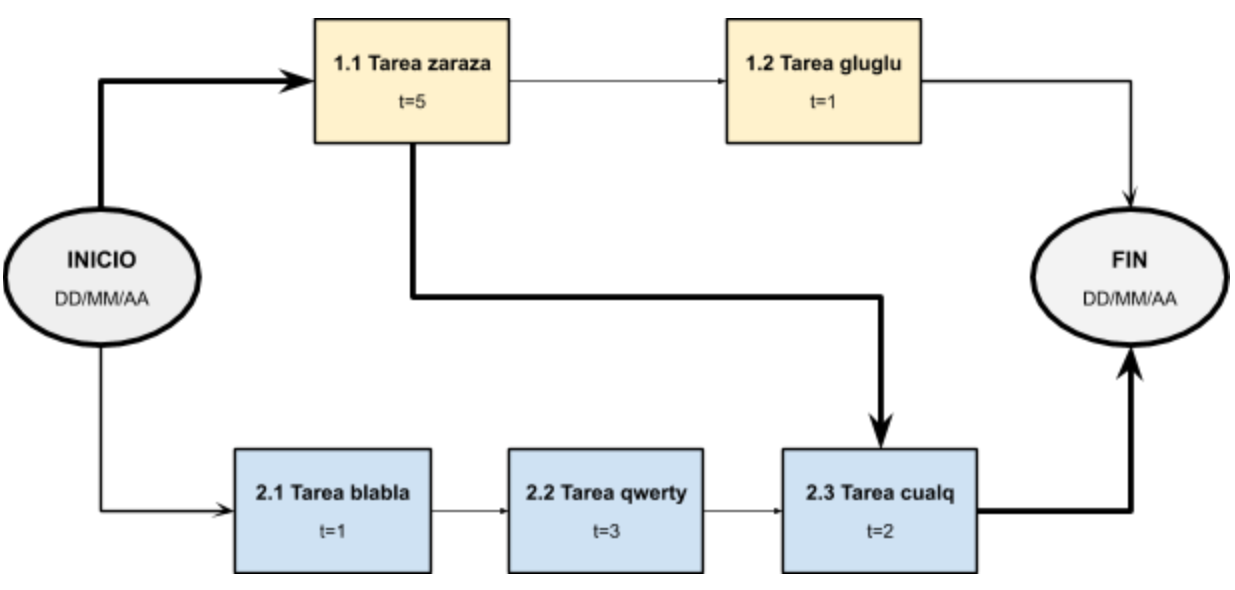
\includegraphics[width=.8\textwidth]{./Figuras/AoN.png}
\caption{Diagrama de \textit{Activity on Node}.}
\label{fig:AoN}
\end{figure}

Indicar claramente en qué unidades están expresados los tiempos.
De ser necesario indicar los caminos semicríticos y analizar sus tiempos mediante un cuadro.
Es recomendable usar colores y un cuadro indicativo describiendo qué representa cada color, como se muestra en el siguiente ejemplo:



\section{11. Diagrama de Gantt}
\label{sec:gantt}

\begin{consigna}{red}

Existen muchos programas y recursos \textit{online} para hacer diagramas de Gantt, entre los cuales destacamos:

\begin{itemize}
\item Planner
\item GanttProject
\item Trello + \textit{plugins}. En el siguiente link hay un tutorial oficial: \\ \url{https://blog.trello.com/es/diagrama-de-gantt-de-un-proyecto}
\item Creately, herramienta online colaborativa. \\\url{https://creately.com/diagram/example/ieb3p3ml/LaTeX}
\item Se puede hacer en latex con el paquete \textit{pgfgantt}\\ \url{http://ctan.dcc.uchile.cl/graphics/pgf/contrib/pgfgantt/pgfgantt.pdf}
\end{itemize}

Pegar acá una captura de pantalla del diagrama de Gantt, cuidando que la letra sea suficientemente grande como para ser legible. 
Si el diagrama queda demasiado ancho, se puede pegar primero la ``tabla'' del Gantt y luego pegar la parte del diagrama de barras del diagrama de Gantt.

Configurar el software para que en la parte de la tabla muestre los códigos del EDT (WBS).\\
Configurar el software para que al lado de cada barra muestre el nombre de cada tarea.\\
Revisar que la fecha de finalización coincida con lo indicado en el Acta Constitutiva.

En la figura \ref{fig:gantt}, se muestra un ejemplo de diagrama de Gantt realizado con el paquete de \textit{pgfgantt}. En la plantilla pueden ver el código que lo genera y usarlo de base para construir el propio.

\begin{figure}[htbp]
\begin{center}
\begin{ganttchart}{1}{12}
  \gantttitle{2020}{12} \\
  \gantttitlelist{1,...,12}{1} \\
  \ganttgroup{Group 1}{1}{7} \\
  \ganttbar{Task 1}{1}{2} \\
  \ganttlinkedbar{Task 2}{3}{7} \ganttnewline
  \ganttmilestone{Milestone o hito}{7} \ganttnewline
  \ganttbar{Final Task}{8}{12}
  \ganttlink{elem2}{elem3}
  \ganttlink{elem3}{elem4}
\end{ganttchart}
\end{center}
\caption{Diagrama de Gantt de ejemplo}
\label{fig:gantt}
\end{figure}


\begin{landscape}
\begin{figure}[htpb]
\centering 
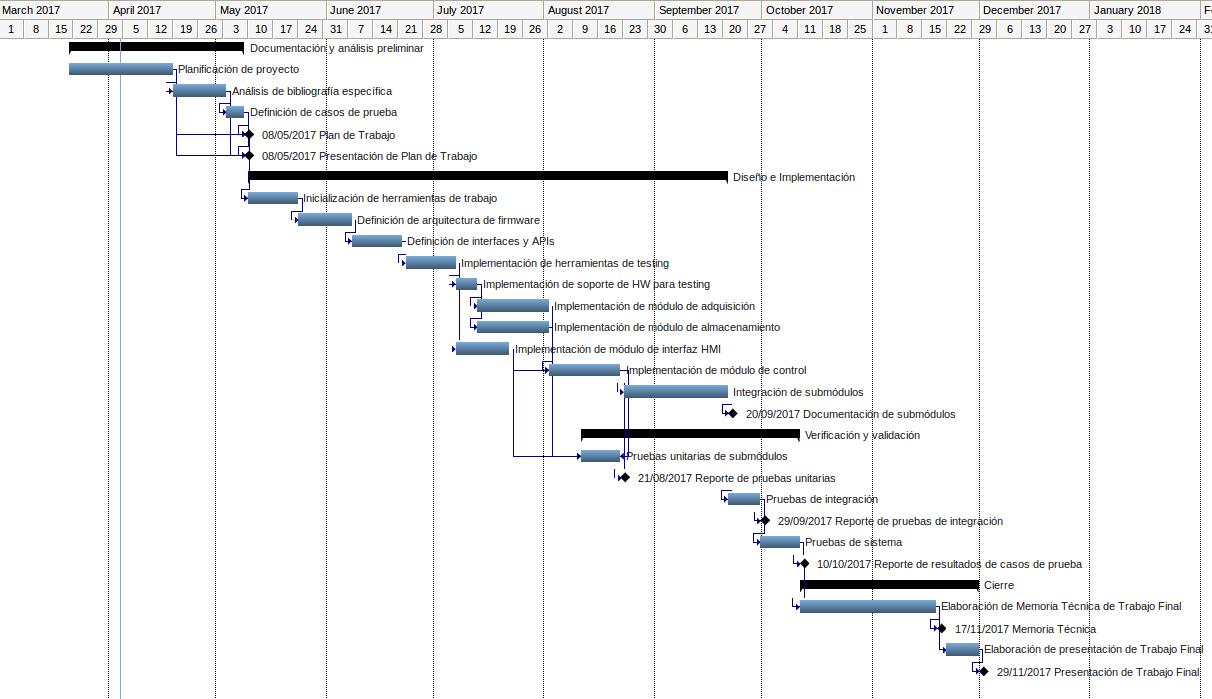
\includegraphics[height=.85\textheight]{./Figuras/Gantt-2.png}
\caption{Ejemplo de diagrama de Gantt rotado}
\label{fig:diagGantt}
\end{figure}

\end{landscape}

\end{consigna}


\section{12. Presupuesto detallado del proyecto}
\label{sec:presupuesto}

\begin{consigna}{red}
Si el proyecto es complejo entonces separarlo en partes:
\begin{itemize}
	\item Un total global, indicando el subtotal acumulado por cada una de las áreas.
	\item El desglose detallado del subtotal de cada una de las áreas.
\end{itemize}

IMPORTANTE: No olvidarse de considerar los COSTOS INDIRECTOS.

\end{consigna}

\begin{table}[htpb]
\centering
\begin{tabularx}{\linewidth}{@{}|X|c|r|r|@{}}
\hline
\rowcolor[HTML]{C0C0C0} 
\multicolumn{4}{|c|}{\cellcolor[HTML]{C0C0C0}COSTOS DIRECTOS} \\ \hline
\rowcolor[HTML]{C0C0C0} 
Descripción &
  \multicolumn{1}{c|}{\cellcolor[HTML]{C0C0C0}Cantidad} &
  \multicolumn{1}{c|}{\cellcolor[HTML]{C0C0C0}Valor unitario} &
  \multicolumn{1}{c|}{\cellcolor[HTML]{C0C0C0}Valor total} \\ \hline
 &
  \multicolumn{1}{c|}{} &
  \multicolumn{1}{c|}{} &
  \multicolumn{1}{c|}{} \\ \hline
 &
  \multicolumn{1}{c|}{} &
  \multicolumn{1}{c|}{} &
  \multicolumn{1}{c|}{} \\ \hline
\multicolumn{1}{|l|}{} &
   &
   &
   \\ \hline
\multicolumn{1}{|l|}{} &
   &
   &
   \\ \hline
\multicolumn{3}{|c|}{SUBTOTAL} &
  \multicolumn{1}{c|}{} \\ \hline
\rowcolor[HTML]{C0C0C0} 
\multicolumn{4}{|c|}{\cellcolor[HTML]{C0C0C0}COSTOS INDIRECTOS} \\ \hline
\rowcolor[HTML]{C0C0C0} 
Descripción &
  \multicolumn{1}{c|}{\cellcolor[HTML]{C0C0C0}Cantidad} &
  \multicolumn{1}{c|}{\cellcolor[HTML]{C0C0C0}Valor unitario} &
  \multicolumn{1}{c|}{\cellcolor[HTML]{C0C0C0}Valor total} \\ \hline
\multicolumn{1}{|l|}{} &
   &
   &
   \\ \hline
\multicolumn{1}{|l|}{} &
   &
   &
   \\ \hline
\multicolumn{1}{|l|}{} &
   &
   &
   \\ \hline
\multicolumn{3}{|c|}{SUBTOTAL} &
  \multicolumn{1}{c|}{} \\ \hline
\rowcolor[HTML]{C0C0C0}
\multicolumn{3}{|c|}{TOTAL} &
   \\ \hline
\end{tabularx}%
\end{table}


\section{13. Gestión de riesgos}
\label{sec:riesgos}

\begin{consigna}{red}
a) Identificación de los riesgos (al menos cinco) y estimación de sus consecuencias:
 
Riesgo 1: detallar el riesgo (riesgo es algo que si ocurre altera los planes previstos de forma negativa)
\begin{itemize}
	\item Severidad (S): mientras más severo, más alto es el número (usar números del 1 al 10).\\
	Justificar el motivo por el cual se asigna determinado número de severidad (S).
	\item Probabilidad de ocurrencia (O): mientras más probable, más alto es el número (usar del 1 al 10).\\
	Justificar el motivo por el cual se asigna determinado número de (O). 
\end{itemize}   

Riesgo 2:
\begin{itemize}
	\item Severidad (S): 
	\item Ocurrencia (O):
\end{itemize}

Riesgo 3:
\begin{itemize}
	\item Severidad (S): 
	\item Ocurrencia (O):
\end{itemize}


b) Tabla de gestión de riesgos:      (El RPN se calcula como RPN=SxO)

\begin{table}[htpb]
\centering
\begin{tabularx}{\linewidth}{@{}|X|c|c|c|c|c|c|@{}}
\hline
\rowcolor[HTML]{C0C0C0} 
Riesgo & S & O & RPN & S* & O* & RPN* \\ \hline
       &   &   &     &    &    &      \\ \hline
       &   &   &     &    &    &      \\ \hline
       &   &   &     &    &    &      \\ \hline
       &   &   &     &    &    &      \\ \hline
       &   &   &     &    &    &      \\ \hline
\end{tabularx}%
\end{table}

Criterio adoptado: 
Se tomarán medidas de mitigación en los riesgos cuyos números de RPN sean mayores a...

Nota: los valores marcados con (*) en la tabla corresponden luego de haber aplicado la mitigación.

c) Plan de mitigación de los riesgos que originalmente excedían el RPN máximo establecido:
 
Riesgo 1: plan de mitigación (si por el RPN fuera necesario elaborar un plan de mitigación).
  Nueva asignación de S y O, con su respectiva justificación:
  - Severidad (S): mientras más severo, más alto es el número (usar números del 1 al 10).
          Justificar el motivo por el cual se asigna determinado número de severidad (S).
  - Probabilidad de ocurrencia (O): mientras más probable, más alto es el número (usar del 1 al 10).
          Justificar el motivo por el cual se asigna determinado número de (O).

Riesgo 2: plan de mitigación (si por el RPN fuera necesario elaborar un plan de mitigación).
 
Riesgo 3: plan de mitigación (si por el RPN fuera necesario elaborar un plan de mitigación).

\end{consigna}


\section{14. Gestión de la calidad}
\label{sec:calidad}

\begin{consigna}{red}
Elija al menos diez requerientos que a su criterio sean los más importantes/críticos/que aportan más valor y para cada uno de ellos indique las acciones de verificación y validación que permitan asegurar su cumplimiento.

\begin{itemize} 
\item Req \#1: copiar acá el requerimiento.

\begin{itemize}
	\item Verificación para confirmar si se cumplió con lo requerido antes de mostrar el sistema al cliente. Detallar 
	\item Validación con el cliente para confirmar que está de acuerdo en que se cumplió con lo requerido. Detallar  
\end{itemize}

\end{itemize}

Tener en cuenta que en este contexto se pueden mencionar simulaciones, cálculos, revisión de hojas de datos, consulta con expertos, mediciones, etc.  Las acciones de verificación suelen considerar al entregable como ``caja blanca'', es decir se conoce en profundidad su funcionamiento interno.  En cambio, las acciones de validación suelen considerar al entregable como ``caja negra'', es decir, que no se conocen los detalles de su funcionamiento interno.

\end{consigna}

\section{15. Procesos de cierre}    
\label{sec:cierre}

\begin{consigna}{red}
Establecer las pautas de trabajo para realizar una reunión final de evaluación del proyecto, tal que contemple las siguientes actividades:

\begin{itemize}
	\item Pautas de trabajo que se seguirán para analizar si se respetó el Plan de Proyecto original:
	 - Indicar quién se ocupará de hacer esto y cuál será el procedimiento a aplicar. 
	\item Identificación de las técnicas y procedimientos útiles e inútiles que se emplearon, y los problemas que surgieron y cómo se solucionaron:
	 - Indicar quién se ocupará de hacer esto y cuál será el procedimiento para dejar registro.
	\item Indicar quién organizará el acto de agradecimiento a todos los interesados, y en especial al equipo de trabajo y colaboradores:
	  - Indicar esto y quién financiará los gastos correspondientes.
\end{itemize}

\end{consigna}


\end{document}
